\documentclass{beamer} 
\usetheme{Berlin}
\usepackage{showexpl} 
\usepackage{tikz}
\usepackage{chemfig}
\usepackage[utf8]{inputenc}

\usepackage{circuitikz}
\usepackage[english]{babel}
\usepackage{blindtext}
\usepackage{multicol}
\usepackage{ragged2e}
\usepackage{pgf-pie}



\title{Latex}
\subtitle{Describe The Document !}



\lstloadlanguages{[LaTeX]Tex} 
\lstset{% 
     basicstyle=\ttfamily\small, 
     commentstyle=\itshape\ttfamily\small, 
     showspaces=false, 
     showstringspaces=false, 
     breaklines=true, 
     breakautoindent=true, 
     captionpos=t 
} 


\begin{document} 


\frame {
		\titlepage
	}

%%%%%%%%%%%%%%%%%%%%%%%%%%%%%%%%%%%%%5

\frame[containsverbatim]{ 
\frametitle{Latex is a Markup Language, like HTML}

\begin{LTXexample} 
\begin{itemize} 
  \item First item 
  \item Second.
  \item Third.
\end{itemize} 
\end{LTXexample} 
 
} 

%%%%%%%%%%%%%%%%%%%%%%%%%%%%%%%%%%%%%%%%%%%%%%

\frame[containsverbatim]
{
\frametitle{but much more powerful ...} 
\begin{LTXexample} 

\begin{align}
\sqrt{37} & = \sqrt{\frac{73^2-1}{12^2}} \\
 & = \sqrt{\frac{73^2}{12^2}\cdot\frac{73^2-1}{73^2}} \\ 
 & = \sqrt{\frac{73^2}{12^2}}\sqrt{\frac{73^2-1}{73^2}} \\
 & \approx \frac{73}{12}\left(1 - \frac{1}{2\cdot73^2}\right)
\end{align}
\end{LTXexample}
} 


%%%%%%%%%%%%%%%%%%%%%%%%%%%%%%%%%%%%%%%%%%

\frame[containsverbatim]
{
\frametitle{Made for Maths but its a multipurpose tool} 
\begin{LTXexample} 
$$  x^2 + y^2 = z^2 $$
$$ \int \frac{x^5 - 4x^3 + 6x}{x}\ dx$$
$$\sum_{i=0}^n i^2 = \frac{(n^2+n)(2n+1)}{6}$$
\end{LTXexample}
} 
%%%%%%%%%%%%%%%%%%%%%%%%%%%%%%%%%%%%%%%






%%%%%%%%%%%%%%%%%%%%%%%%%%%%%%%%%%%%%5

\frame[containsverbatim]{ 
\frametitle{Shades and Colours are easy and quick}

\begin{LTXexample} 

\begin{tikzpicture}
\shade (0,0) circle (.5cm); 
\end{tikzpicture}
\end{LTXexample} 
 
\begin{LTXexample} 

\begin{tikzpicture}
\fill[blue!40!white] (0,0) rectangle (5,2);
\end{tikzpicture}
\end{LTXexample} 



} 

%%%%%%%%%%%%%%%%%%%%%%%%%%%%%%%%%%%%%%%%%%%%%%


\frame[containsverbatim]{ 
\frametitle{Even Gradient ..}

\begin{LTXexample} 

\begin{tikzpicture}
\shade[left color=red,right color=yellow]
(0,0) rectangle (5,4);
\end{tikzpicture}
\end{LTXexample}
 
} 

%%%%%%%%%%%%%%%%%%%%%%%%%%%%%%%%%%%%%%%%


\frame[containsverbatim]{ 
\frametitle{Inner and Outer Gradient ..}

\begin{LTXexample} 
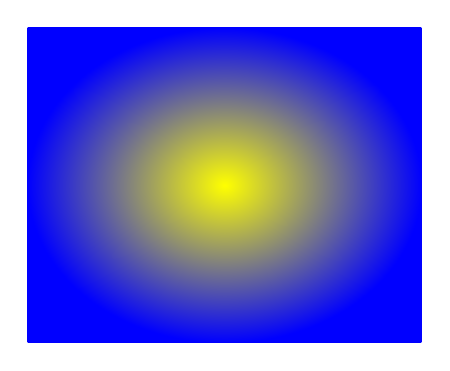
\begin{tikzpicture}
\shade[inner color=yellow,outer color=blue] (0,0) rectangle (5,4);
\end{tikzpicture}
\end{LTXexample}
 
} 



%%%%%%%%%%%%%%%%%%%%%%%%%%%%%%%%%%%%%%%%%%%

\frame
{
\frametitle{Seamless Graphics and Text mixture } 
\section{ }
Question : The slant height of a right circular cone is 3 cm. Find the height of cone, if its volume is the greatest.\\
%----------------------------------------
\vspace{0.4cm}
Solution : Let r  and x  be the base-radius and the height of the cone respectively. Then volume of the cone f(x) is given by

\begin{equation} \nonumber
\begin{alignedat}{4}
f(x) &= \frac{1}{3}\pi r^2x\\
&= \frac{\pi}{3}(3^2-x^2)x\\
&= \frac{\pi}{3}(9x - x^3)\\
\therefore f'(x) &=  \frac{\pi}{3}(9 - 3x^2)\\
\end{alignedat}
%\vrule
\quad\quad\quad
\begin{alignedat}{4}
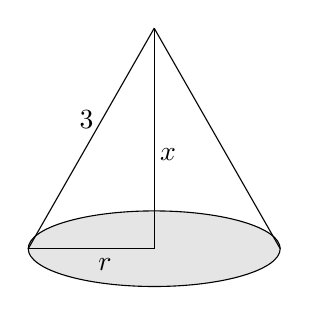
\begin{tikzpicture}[scale=0.8]
\filldraw[fill=gray!20](0,0) ellipse (2cm and 0.6cm);
\draw (0,0) -- node[below] {\ \ \ $x$}(0,3.5);
\draw (0,0)  -- node[below] {\ \ \ $r$} (-2,0);
\draw  (-2,0) --node[above] {3\ \ }(0,3.5);
\draw  (2,0) -- (0,3.5);
\end{tikzpicture}\\\\
\end{alignedat}
\end{equation}
}


%%%%%%%%%%%%%%%%%%%%%%%%%%%%%%%%%%%%%

\frame[containsverbatim]{ 
\frametitle{Chemical Formulae with Package 'chemfig' }

\verb|\chemfig{O=H}   will give    |  \chemfig{O=H}\\~\\

Default angle units : 1 unit = 45$^{\circ}$. Hence in the following example, the angles are 45$^{\circ}$ and 315$^{\circ}$. \\~\\

\verb| \chemfig{H_3C-CH_2(-[2]CH_3)-C(=[1]O)-[7]O-CH_3} gives|  
 \\~\\
\chemfig{H_3C-CH_2(-[2]CH_3)-C(=[1]O)-[7]O-CH_3}
 
} 

%%%%%%%%%%%%%%%%%%%%%%%%%%%%%%%%%%%%%%%






%%%%%%%%%%%%%%%%%%%%%%%%%%%%%%%%%%%%%

\frame[containsverbatim]
{
\frametitle{Chemical Formulae with Package 'chemfig'} 
\begin{LTXexample} 
\vspace{5mm}
\chemfig{A*6(-B=C(-CH_3)-D-E-F(=G)=)}
\vspace{5mm}
\end{LTXexample}
} 

%%%%%%%%%%%%%%%%%%%%%%%%%%%%%%%%%%%%%%%







%%%%%%%%%%%%%%%%%%%%%%%%%%%%%%%%%%%%%

\frame[containsverbatim]{ 
\frametitle{Physics Circuits with Package 'circuitikz' }

\begin{circuitikz}[american voltages]
\draw
  (0,0) to [short, *-] (6,0)
  to [V, l_=$\mathrm{j}{\omega}_m \underline{\psi}^s_R$] (6,2) 
  to [R, l_=$R_R$] (6,4) 
  to [short, i_=$\underline{i}^s_R$] (5,4) 
  (0,0) to [open, v^>=$\underline{u}^s_s$] (0,4) 
  to [short, *- ,i=$\underline{i}^s_s$] (1,4) 
  to [R, l=$R_s$] (3,4)
  to [L, l=$L_{\sigma}$] (5,4) 
  to [short, i_=$\underline{i}^s_M$] (5,3) 
  to [L, l_=$L_M$] (5,0); 
  (0,0) to[nos] (8,0); 
  \end{circuitikz}
 
} 

%%%%%%%%%%%%%%%%%%%%%%%%%%%%%%%%%%%%%%%



%%%%%%%%%%%%%%%%%%%%%%%%%%%%%%%%%%%%%



%%%%%%%%%%%%%%%%%%%%%%%%%%%%%%%%%%%%%%%






%%%%%%%%%%%%%%%%%%%%%%%%%%%%%%%%%%%%%

\frame[containsverbatim]{ 
\frametitle{Pie Chart }

\begin{LTXexample} 
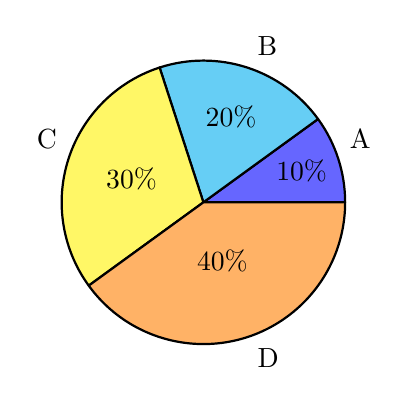
\begin{tikzpicture}[scale=0.6]
    \pie{10/A, 20/B, 30/C, 40/D}
\end{tikzpicture}
\end{LTXexample}

} 

%%%%%%%%%%%%%%%%%%%%%%%%%%%%%%%%%%%%%%%



%%%%%%%%%%%%%%%%%%%%%%%%%%%%%%%%%%%%%

\frame[containsverbatim]{ 
\frametitle{Programming inside your document }
\begin{LTXexample} 
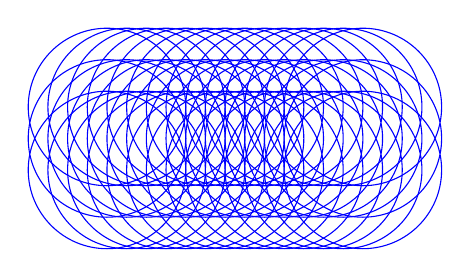
\begin{tikzpicture}
\foreach \n in {0,...,13}
      \draw [blue]
         (\n/4,0.4) circle [radius = 1]
         (\n/4,0) circle [radius = 1]
         (\n/4,-0.4) circle [radius = 1] ;
\end{tikzpicture}
\end{LTXexample} 
} 

%%%%%%%%%%%%%%%%%%%%%%%%%%%%%%%%%%%%%%%





%%%%%%%%%%%%%%%%%%%%%%%%%%%%%%%%%%%%%

\frame[containsverbatim]{ 
\frametitle{Three Column Magazine Format For Book Publishers }

% column divider
%\setlength\columnseprule{0.5pt}


\begin{multicols}{3}
\justify
\blindtext
\end{multicols}

 
} 

%%%%%%%%%%%%%%%%%%%%%%%%%%%%%%%%%%%%%%%




\end{document}